% questions.tex —— 1977 年·广西卷（理科） · 题目内容片段（无答案）
% 由 tools/generate_projects.py 依来源总账自 1977/1977_数学真题_广西理_试题.md 生成，勿手改（改源 MD 后重跑）


\gkpart{数学试题解（广西卷·理科）}

\begin{gktip}
\textbf{来源说明}：本题面依据固定源 PDF《广西1977年高考数学试题解（理科）》第 1—6 页逐题转录。源 PDF 是题面与解答连排的《试题解》扫描材料（书页 107—111 及无页码续页），每题题面后紧跟源解答。正式题共五道：第一大题含 5 个小题（每小题 5 分，本题 25 分），第二题 20 分，第三题 17 分，第四题 18 分，第五题 20 分，合计 100 分。源卷在第五题后印有「〔选作题〕考生可根据自己能力选作，作为参考成绩，不列入总分」，其下两道选作题沿用大题号「一、二」，本库按参考题 1、2 处理，不计入正式题量。原卷大题号「一、二、三、四、五」转写为主观题号 1—5，第一大题下印作「1．—5．」的五道小题重排为小问（1）—（5）。扫描件存在背面透印文字，与卷面内容无关。
\end{gktip}

\par\medskip

\begin{question}
\gkti{1}\textbf{（每小题 5 分，本题 25 分）} 

\begin{gktip}
\textbf{题号说明}：源卷第一大题下的五道小题印作「1．—5．」，本库规范要求小问连续编号，故重排为（1）—（5），未增删任何题干内容。
\end{gktip}

（1） $x$ 为何值时，$\dfrac{|x|}{x}$ 的值是？是 $-1$？没有意义？

\begin{gktip}
\textbf{源注}：原卷印作「的值是？」，第一个问句疑漏排数值「1」（源解答应为「的值是 1？」）；本文按原卷保留。
\end{gktip}

（2） 不查表求：$\lg 2-2\lg 4+\lg 5+\lg 16$ 的值。

（3） 计算：$\operatorname{ctg}(-60^\circ)\sin 240^\circ-2\cos(-60^\circ)+\operatorname{tg}^2 150^\circ$。

（4） 计算：$\left(-1\dfrac12\right)^2+81^{\frac34}-(-1)^0\div 0.2+(-2)^{-3}$。

\begin{gktip}
\textbf{源注}：原卷 $(-1)$ 的指数印作小圆圈「°」，源解答按零次幂处理；本文转录为 $(-1)^0$。
\end{gktip}

（5） 求 $A(7,5)$ 和 $B(1,-3)$ 两点间的距离。

\end{question}
\begin{question}
\gkti{2}\textbf{（20 分）} 红旗机械厂生产 360 台车床，原计划若干天完成，在党的十一大精神舞午下，实际每天比原计划多生产 12 台，结果提前 8 天完成任务。问实际每天生产多少台车床？

\begin{gktip}
\textbf{源注}：原卷印作「精神舞午下」，当为「精神鼓舞下」之误排；本文按原卷保留。
\end{gktip}

\Needspace{0.4\textheight}
\end{question}
\begin{question}
\gkti{3}\textbf{（17 分）} 在四边形 $ABCD$ 中，$E\text{、}F$ 分别是对角线 $AC\text{、}BD$ 的中点，$M\text{、}N$ 分别是 $AB\text{、}CD$ 的中点，求证 $EF$ 与 $MN$ 互相平分。
\nopagebreak[4]
\begin{center}% 1977 年广西卷（理科）第 3 题：四边形 ABCD，E、F 为对角线 AC、BD 的中点，M、N 为 AB、CD 的中点，
% 虚线四边形 EMFN 为平行四边形，MN、EF 是其对角线（按源卷第 2 页布局）
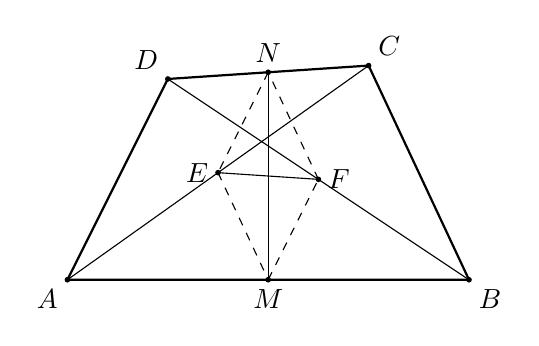
\begin{tikzpicture}[scale=0.85]
  \coordinate (A) at (0,0);
  \coordinate (B) at (6,0);
  \coordinate (D) at (1.5,3);
  \coordinate (C) at (4.5,3.2);
  \coordinate (M) at (3,0);
  \coordinate (N) at (3,3.1);
  \coordinate (E) at (2.25,1.6);
  \coordinate (F) at (3.75,1.5);
  \draw[thick] (A)--(B)--(C)--(D)--cycle;
  \draw[thin] (A)--(C);
  \draw[thin] (B)--(D);
  \draw (E)--(F);
  \draw (M)--(N);
  \draw[dashed] (E)--(M) (M)--(F) (F)--(N) (N)--(E);
  \fill (A) circle (1.2pt) node[below left] {$A$};
  \fill (B) circle (1.2pt) node[below right] {$B$};
  \fill (C) circle (1.2pt) node[above right] {$C$};
  \fill (D) circle (1.2pt) node[above left] {$D$};
  \fill (M) circle (1.2pt) node[below] {$M$};
  \fill (N) circle (1.2pt) node[above] {$N$};
  \fill (E) circle (1.2pt) node[left] {$E$};
  \fill (F) circle (1.2pt) node[right] {$F$};
\end{tikzpicture}
\end{center}
\nopagebreak[4]
\Needspace{0.4\textheight}
\end{question}
\begin{question}
\gkti{4}\textbf{（18 分）} 已知正四棱锥底面边长为 $6$ 厘米，侧棱是高的 $2$ 倍。求这棱锥的体积。（精确到 $0.1$ 立方厘米）
\nopagebreak[4]
\begin{center}% 1977 年广西卷（理科）第 4 题：正四棱锥 V-ABCD，O 为底面正方形中心（高的垂足），
% 实线：可见侧棱 VA、VB、VC 与底边 AB、BC；虚线：侧棱 VD、底边 AD、DC、高 VO、底面对角线半段 AO、DO（按源卷第 3 页布局）
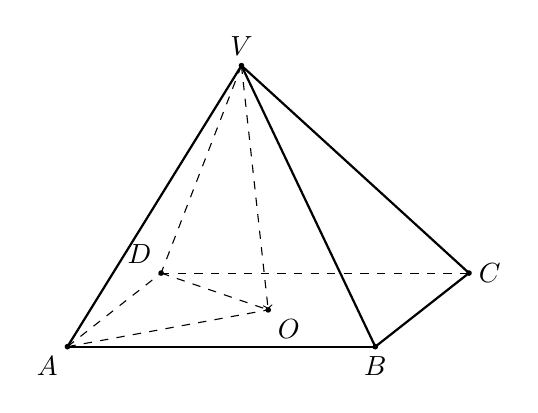
\begin{tikzpicture}[scale=0.85]
  \coordinate (A) at (0,0);
  \coordinate (B) at (4.6,0);
  \coordinate (C) at (6,1.1);
  \coordinate (D) at (1.4,1.1);
  \coordinate (O) at (3,0.55);
  \coordinate (V) at (2.6,4.2);
  \draw[thick] (V)--(A);
  \draw[thick] (V)--(B);
  \draw[thick] (V)--(C);
  \draw[thick] (A)--(B);
  \draw[thick] (B)--(C);
  \draw[dashed] (V)--(D);
  \draw[dashed] (A)--(D);
  \draw[dashed] (D)--(C);
  \draw[dashed,->] (V)--(O);
  \draw[dashed] (A)--(O);
  \draw[dashed] (D)--(O);
  \fill (A) circle (1.2pt) node[below left] {$A$};
  \fill (B) circle (1.2pt) node[below] {$B$};
  \fill (C) circle (1.2pt) node[right] {$C$};
  \fill (D) circle (1.2pt) node[above left] {$D$};
  \fill (O) circle (1.2pt) node[below right] {$O$};
  \fill (V) circle (1.2pt) node[above] {$V$};
\end{tikzpicture}
\end{center}
\nopagebreak[4]
\Needspace{0.4\textheight}
\end{question}
\begin{question}
\gkti{5}\textbf{（20 分）} 把一块钢板冲成上面是半园形、下面是矩形的零件，已知零件的周长是 $P$，怎样才能使冲出的零件面积最大？
\nopagebreak[4]
\begin{center}% 1977 年广西卷（理科）第 5 题：上部半园、下部矩形的零件，矩形宽 x 标于底边下方（按源卷第 3 页布局）
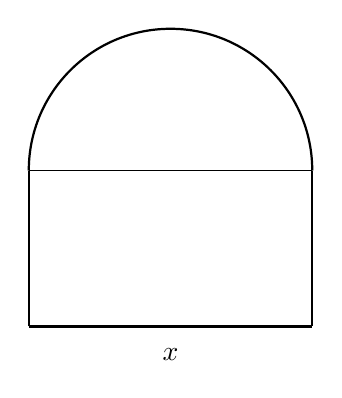
\begin{tikzpicture}[scale=0.9]
  \draw[thick] (0,0)--(4,0);
  \draw[thick] (0,0)--(0,2.2);
  \draw[thick] (4,0)--(4,2.2);
  \draw[thin] (0,2.2)--(4,2.2);
  \draw[thick] (0,2.2) arc(180:0:2);
  \node at (2,-0.4) {$x$};
\end{tikzpicture}
\end{center}
\nopagebreak[4]
\begin{gktip}
\textbf{参考题说明}：源卷第五题后印有「〔选作题〕考生可根据自己能力选作，作为参考成绩，不列入总分」，其下两题沿用大题号「一、二」编号。本库改题为参考题 1、2，不计入正式题量。
\end{gktip}

\Needspace{5\baselineskip}
\textbf{参考题 1．} 解方程组

\nopagebreak[4]
\[
\begin{cases}
\sqrt[3]{(x+y)^2}+2\sqrt[3]{(x-y)^2}=3\sqrt[3]{x^2-y^2},\\
3x-2y=13.
\end{cases}
\]

\textbf{参考题 2．} 线段 $AB$ 之三等分点依次为 $C\text{、}D$，以 $CD$ 为直径画园，在园周上任取一点 $P$。求证 $\operatorname{tg}\angle APC\cdot\operatorname{tg}\angle BPD=\dfrac14$。
\nopagebreak[4]
\begin{center}% 1977 年广西卷（理科）参考题 2：线段 AB 上 C、D 为三等分点，以 CD 为直径作园，P 为园周上一点，
% PE 垂直 AB 于 E，θ 为 PC 与 CD 的夹角（按源卷第 5 页布局）
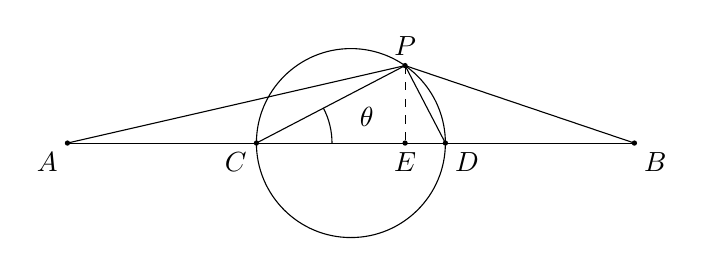
\begin{tikzpicture}[scale=0.8]
  \coordinate (A) at (0,0);
  \coordinate (C) at (3,0);
  \coordinate (D) at (6,0);
  \coordinate (B) at (9,0);
  \coordinate (P) at (5.36,1.23);
  \coordinate (E) at (5.36,0);
  \draw (A)--(B);
  \draw (4.5,0) circle (1.5);
  \draw (A)--(P);
  \draw (B)--(P);
  \draw (P)--(C);
  \draw (P)--(D);
  \draw[dashed] (P)--(E);
  \draw (4.2,0) arc(0:27.5:1.2);
  \node at (4.75,0.42) {$\theta$};
  \fill (A) circle (1.2pt) node[below left] {$A$};
  \fill (B) circle (1.2pt) node[below right] {$B$};
  \fill (C) circle (1.2pt) node[below left] {$C$};
  \fill (D) circle (1.2pt) node[below right] {$D$};
  \fill (E) circle (1.2pt) node[below] {$E$};
  \fill (P) circle (1.2pt) node[above] {$P$};
\end{tikzpicture}
\end{center}
\nopagebreak[4]

\end{question}